\chapter{Módulo: Auditoría}
\label{mod:16-auditoria}

\section{Propósito}
\label{sec:auditoria-proposito}

Bitácora consultable de las operaciones sensibles del sistema: quién hizo qué, cuándo, desde qué dirección IP y sobre qué recurso. Responde a la pregunta de control interno que el registro de \code{CreatedAt}/\code{UpdatedAt} de cada tabla no puede responder --- ese registro dice \emph{cuándo se tocó una fila por última vez}, pero no deja rastro de los eventos que no modifican datos (un inicio de sesión fallido) ni de quién ejecutó una operación que después se revirtió.

Es un módulo transversal: no tiene un flujo de negocio propio, sino que se engancha en los flujos de los demás módulos.

\section{Entidades principales}
\label{sec:auditoria-entidades}

\begin{longtable}{p{3.6cm}p{9.7cm}}
\caption{Entidades principales del módulo de Auditoría.}\label{tab:auditoria-entidades}\\
\toprule
\textbf{Entidad} & \textbf{Rol} \\
\midrule
\endfirsthead
\toprule
\textbf{Entidad} & \textbf{Rol} \\
\midrule
\endhead
\bottomrule
\endfoot
\code{Registro}\allowbreak \code{Auditoria} & Registro \emph{append-only} de un evento auditado (tabla \code{registros_}\allowbreak \code{auditoria}). Campos: \code{FechaHora} (UTC), \code{Categoria}, \code{Accion}, \code{UserId} (nullable), \code{Usuario}\allowbreak \code{Nombre}, \code{Entidad}/\code{EntidadId} (nullables), \code{Descripcion}, \code{SucursalId}, \code{IpAddress}. \\
\code{AuditCategoria} & Enum de agrupación de alto nivel para el filtro de la vista: \code{Seguridad}, \code{Admin}, \code{Operativo}. \\
\code{AuditAccion} & Enum-catálogo de las acciones auditables (15 en esta versión). \\
\code{AuditCatalog} & Clase estática con el mapa único acción $\to$ categoría (\code{Categoria}\allowbreak \code{De}) --- fuente de verdad para clasificar un evento y para poblar el filtro de la vista. \\
\end{longtable}

\section{Reglas de negocio clave}
\label{sec:auditoria-reglas}

\begin{itemize}
  \item \textbf{Captura curada y explícita, no automática.} No hay interceptor de \code{SaveChanges} ni trigger en la base: cada evento auditable llama a \code{IAudit}\allowbreak \code{Service.}\allowbreak \code{LogAsync(.}\allowbreak \code{.}\allowbreak \code{.)} desde el servicio de negocio correspondiente. La decisión es deliberada --- un interceptor genérico registraría \emph{cada} escritura del sistema, produciendo un volumen que nadie audita; el objetivo es una bitácora que un administrador pueda leer, no un \emph{changelog} exhaustivo. Ver \hyperref[adr:0013]{ADR 0013}.
  \item \textbf{El registro se escribe después de la operación de negocio, en su propia transacción.} \code{LogAsync} hace su propio \code{SaveChangesAsync}, de modo que una falla al auditar no revierte la operación auditada, y no se audita una operación que no llegó a persistirse.
  \item \textbf{Append-only y sin navegaciones de dominio.} \code{Registro}\allowbreak \code{Auditoria} no tiene propiedades de navegación: guarda un \emph{snapshot} legible del autor (\code{Usuario}\allowbreak \code{Nombre}) en vez de una FK a \code{User}. Así el historial sigue siendo legible aunque el usuario se renombre o se desactive, y ninguna FK impide borrar un registro padre. No hay endpoint de edición ni de borrado.
  \item \textbf{Los enums se persisten como \code{string}}, única excepción a la convención \code{Has}\allowbreak \code{Conversion<int>()} del resto del modelo (Capítulo~\ref{sec:modelo-datos}). El motivo es operativo: agregar una acción auditable nueva no requiere migración, y la tabla queda legible al consultarla directamente por SQL.
  \item \textbf{La categoría no se pasa como parámetro, se deriva.} \code{LogAsync} recibe solo la acción y obtiene la categoría de \code{AuditCatalog.}\allowbreak \code{CategoriaDe} --- no puede quedar un evento clasificado de forma inconsistente entre dos llamadas.
  \item \textbf{Un inicio de sesión fallido también se audita}, y es el caso que justifica que \code{UserId} sea nullable: si el correo intentado no corresponde a ningún usuario no hay a quién referenciar, así que \code{Usuario}\allowbreak \code{Nombre} guarda el correo tal como se intentó.
  \item \textbf{Acceso restringido al permiso \code{ver_usuarios}}, el mismo que gobierna la administración de usuarios --- la bitácora es una herramienta de administración, no de operación diaria.
\end{itemize}

\subsection{Acciones auditadas}
\label{sec:auditoria-acciones}

\begin{longtable}{p{2.4cm}p{4.4cm}p{6.6cm}}
\caption{Las 15 acciones auditadas y el servicio que las registra.}\label{tab:auditoria-acciones}\\
\toprule
\textbf{Categoría} & \textbf{Acción} & \textbf{Origen} \\
\midrule
\endfirsthead
\toprule
\textbf{Categoría} & \textbf{Acción} & \textbf{Origen} \\
\midrule
\endhead
\bottomrule
\endfoot
Seguridad & \code{LoginExitoso} & \code{AuthService} \\
Seguridad & \code{LoginFallido} & \code{AuthService} --- guarda el correo intentado \\
Seguridad & \code{Password}\allowbreak \code{Cambiado} & \code{AuthService} \\
Seguridad & \code{Password}\allowbreak \code{Reseteado} & \code{UserService} --- reseteo por administrador \\
Admin & \code{Usuario}\allowbreak \code{Desactivado} & \code{UserService} \\
Admin & \code{RolAsignado} & \code{RoleService} \\
Admin & \code{RolQuitado} & \code{RoleService} \\
Admin & \code{RolCreado} & \code{RoleService} \\
Admin & \code{RolActualizado} & \code{RoleService} \\
Admin & \code{RolEliminado} & \code{RoleService} \\
Operativo & \code{VentaAnulada} & \code{VentaService} \\
Operativo & \code{Devolucion}\allowbreak \code{Aprobada} & \code{VentaService} \\
Operativo & \code{Devolucion}\allowbreak \code{Rechazada} & \code{VentaService} \\
Operativo & \code{CierreCaja}\allowbreak \code{Aprobado} & \code{CajaService} \\
Operativo & \code{CierreCaja}\allowbreak \code{Rechazado} & \code{CajaService} \\
\end{longtable}

Quedan fuera de esta versión, de forma consciente: el alta y la edición de usuarios (que hoy ocurren a través de los servicios de \code{Professional}/\code{Patient}), los cambios de precio o costo de un producto y los ajustes manuales de stock.

\section{Endpoints}
\label{sec:auditoria-endpoints}

Detalle completo en el Apéndice de Referencia de API, \S 15 (\code{Auditoria}\allowbreak \code{Controller}).

\begin{longtable}{p{1.6cm}p{5.6cm}p{6.4cm}}
\caption{Endpoints del módulo de Auditoría.}\label{tab:auditoria-endpoints}\\
\toprule
\textbf{Método} & \textbf{Ruta} & \textbf{Descripción} \\
\midrule
\endfirsthead
\toprule
\textbf{Método} & \textbf{Ruta} & \textbf{Descripción} \\
\midrule
\endhead
\bottomrule
\endfoot
GET & \texttt{/api/auditoria?}\allowbreak \texttt{categoria\&accion\&}\allowbreak \texttt{userId\&fechaDesde\&}\allowbreak \texttt{fechaHasta\&search\&}\allowbreak \texttt{page\&pageSize} & Bitácora paginada (20 por página por defecto, máximo 100), ordenada de más reciente a más antiguo. \code{search} busca en descripción y nombre de usuario (\code{ILIKE}). \\
GET & \texttt{/api/auditoria/acciones} & Catálogo de acciones con su categoría, para poblar el filtro del frontend sin duplicar la lista. \\
\end{longtable}

Ambos exigen la policy \code{ver_usuarios}. No existe \code{POST}, \code{PUT} ni \code{DELETE}: la bitácora se escribe únicamente desde adentro del sistema.

\section{Flujo típico}
\label{sec:auditoria-flujo}

\begin{figure}[htbp]
\centering
\begin{tikzpicture}[node distance=1.3cm]
  \node[actor] (svc) {VentaService\\(u otro)};
  \node[actor, right=of svc] (aud) {AuditService};
  \node[actor, right=of aud] (db) {PostgreSQL};
  \node[actor, right=of db] (view) {Auditoria\\View};

  \draw[lineavida] (svc.south) -- ++(0,-7.9);
  \draw[lineavida] (aud.south) -- ++(0,-7.9);
  \draw[lineavida] (db.south) -- ++(0,-7.9);
  \draw[lineavida] (view.south) -- ++(0,-7.9);

  \draw[mensaje] ($(svc.south)+(0,-1.5)$) -- node[above,font=\scriptsize,align=center,fill=white,inner sep=1.5pt]{operación de negocio (anular venta)} ($(db.south)+(0,-1.5)$);
  \draw[mensaje] ($(svc.south)+(0,-2.8)$) -- node[above,font=\scriptsize,align=center,fill=white,inner sep=1.5pt]{LogAsync(VentaAnulada,\\descripción, entidad, id)} ($(aud.south)+(0,-2.8)$);
  \draw[mensaje] ($(aud.south)+(0,-4.0)$) -- node[above,font=\scriptsize,align=center,fill=white,inner sep=1.5pt]{INSERT registros\_auditoria\\(SaveChanges propio)} ($(db.south)+(0,-4.0)$);
  \draw[mensaje] ($(view.south)+(0,-5.5)$) -- node[above,font=\scriptsize,align=center,fill=white,inner sep=1.5pt]{GET /api/auditoria\\(filtros + paginación)} ($(aud.south)+(0,-5.5)$);
  \draw[mensaje] ($(aud.south)+(0,-6.7)$) -- node[above,font=\scriptsize,align=center,fill=white,inner sep=1.5pt]{SELECT paginado} ($(db.south)+(0,-6.7)$);
  \draw[mensajeretorno] ($(db.south)+(0,-7.6)$) -- node[below,font=\scriptsize,fill=white,inner sep=1.5pt]{página de registros} ($(view.south)+(0,-7.6)$);
\end{tikzpicture}
\caption{La escritura de la bitácora es un paso explícito y posterior a la operación de negocio, con su propia transacción: si falla el registro de auditoría, la operación auditada ya quedó persistida.}
\label{fig:seq-auditoria}
\end{figure}

\section{Vistas de frontend}
\label{sec:auditoria-vistas}

\begin{itemize}
  \item \code{AuditoriaView.vue} (\code{/admin/auditoria}) --- tabla de registros con filtro por categoría (\code{FilterChips} de valor único), selector de acción agrupado por categoría, rango de fechas y búsqueda de texto libre. La paginación es del lado del servidor, reutilizando el componente \code{Pagination}\allowbreak \code{Footer} común.
  \item \code{services/}\allowbreak \code{auditoriaService.}\allowbreak \code{ts} --- cliente HTTP más los diccionarios \code{ACCION_}\allowbreak \code{LABELS} y \code{CATEGORIA_}\allowbreak \code{LABELS}, que traducen los valores del enum a etiquetas en español para la interfaz.
\end{itemize}

\section{Interfaz}
\label{sec:auditoria-interfaz}

\begin{figure}[htbp]
\centering
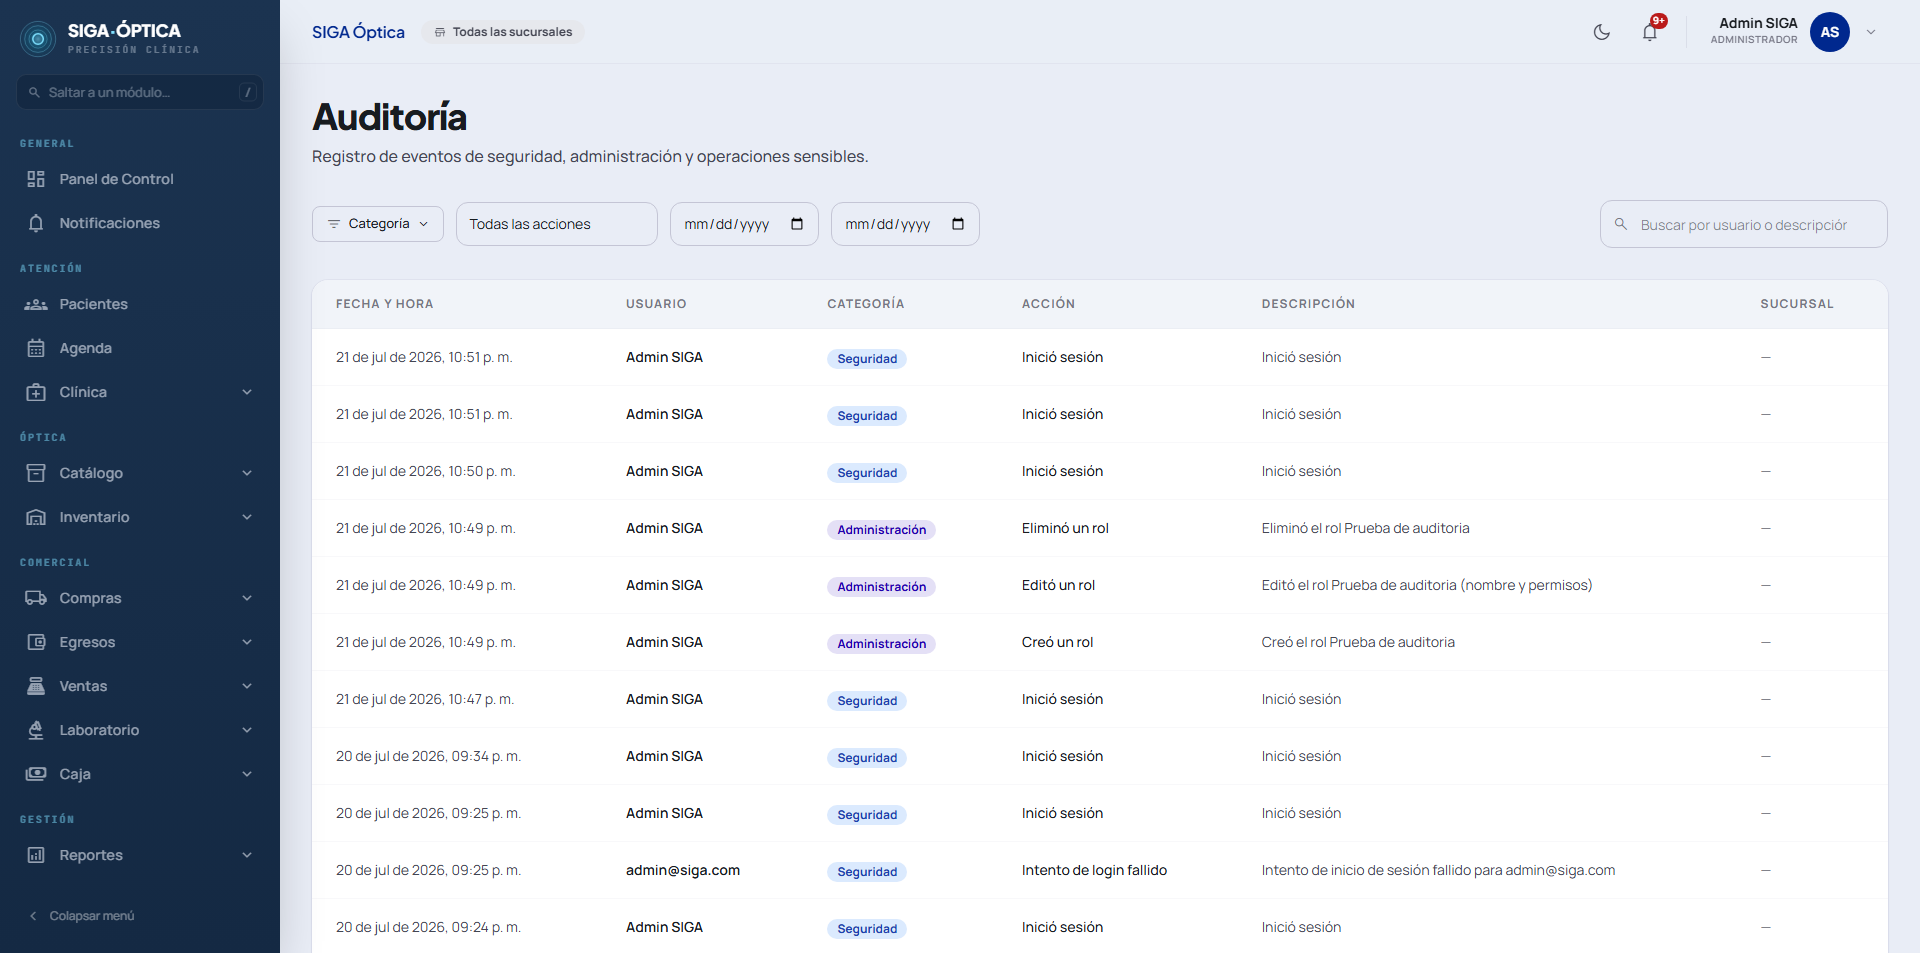
\includegraphics[width=0.95\textwidth]{imagenes/mod16-auditoria.png}
\caption{Bitácora de auditoría con los filtros por categoría, acción, rango de fechas y texto libre. Cada registro muestra la fecha y hora, el usuario responsable, la categoría, la acción y una descripción legible; el intento de inicio de sesión fallido es el caso que justifica que el usuario se guarde como texto y no como clave foránea.}
\label{fig:mod16-auditoria}
\end{figure}

\section{Estado}
\label{sec:auditoria-estado}

\Implementado\ (backend \code{AuditService} + \code{Auditoria}\allowbreak \code{Controller} + entidad \code{Registro}\allowbreak \code{Auditoria}, migración \code{066_}\allowbreak \code{Registro}\allowbreak \code{Auditoria}; frontend \code{auditoriaService.}\allowbreak \code{ts} + \code{AuditoriaView.}\allowbreak \code{vue}). Reemplazó al marcador de posición que ocupaba antes esa entrada del menú.
